\chapter{SLAM}\label{chp:slam_mapping}

One of the first challenges in indoor navigation for assistive robots is actually finding where they are. Robot localization is fundamental to not only know where you need to go, but rather find a path there that avoids the obstacles.

Mapping is an essential tool in this matter, and it comprises the areas of \textit{concurrent mapping} and \textit{localization problem}. On themselves, both problems are relatively easy and well understood: mapping an environment knowing the localization and localizing the robot having the map in hands are simple tasks, however the combination of those two problems is hard to solve \cite{thrun2000real}.

Many SLAM (Simultaneous Localization and
Map Building) algorithms emerged to try and solve these problems, using different approaches and range of sensors to do the task. Some even evolved fusing data from different sensors to provide higher precision. They often rely on assumptions about the system nature. Most of the algorithms assume that the noise can be modeled  as a gaussian. Others might assume that the movement is linear and apply Kalman Filters to predict the current state.

\section{Sensors}

\subsection{Laser Scanners}

The laser scanner is one of the most simple ways to capture data about the environment. They work by sending beams of light in a direction and measuring the time it takes for the light to travel back and forth between the object and the sensor. As you want information to be gathered on more than a single point, the scanner can rotate a mirror or even the whole sensor to gather measurements from all directions, as shown on \prettyref{fig:sick_s300_diagram}. There are two main ways of measuring the object distance: time of flight and Phase-Shift \cite{amann2001laser}.

\begin{figure}
     \centering
     \subfloat[][]{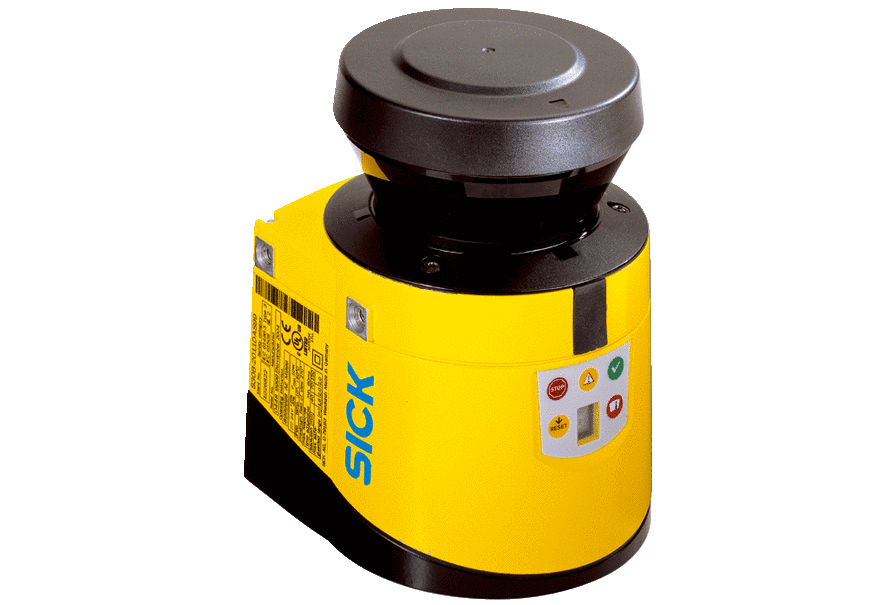
\includegraphics[width=80mm]{sick_s300}}
     \subfloat[][]{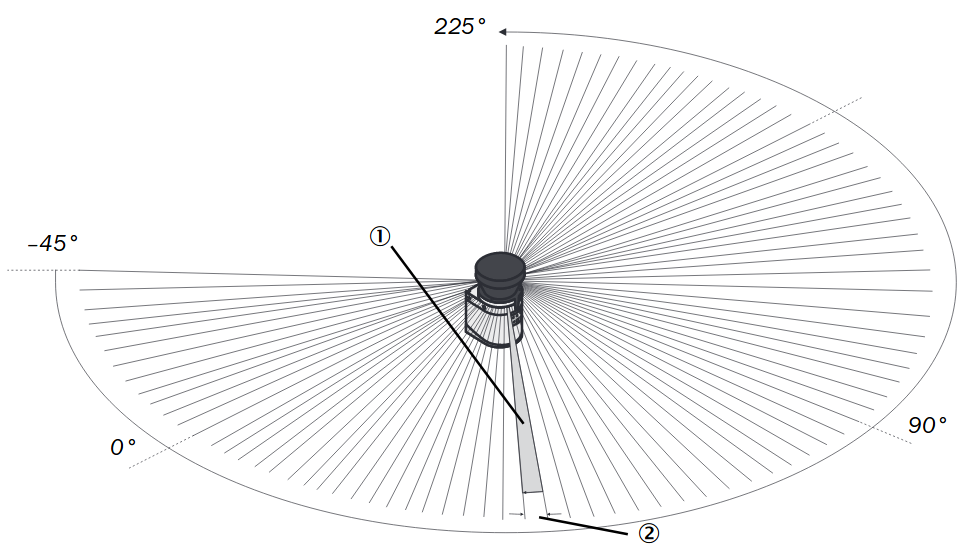
\includegraphics[width=80mm]{sick_s300_diagram}\label{fig:sick_s300_diagram}}
     \caption{SICK S300 Laser Scanner \cite{sicks300}.}
     \label{fig:sick_s300}
\end{figure}

In the time of flight measurement, a stopwatch is started when the beam of light is emitted. Since the speed of light is well known, the calculations are very straight forward, as shown on \prettyref{eq:d}. This form of measurement depends heavily on the quality of construction, as the usual sources of inaccuracy are noise (electronics, radiation in the room), timing (stopwatch precision, pulse detection), and minimal changes in each measurement can lead to big errors in the final result. Averaging and Filtering also take a big role in providing reliable data.

\begin{equation} \label{eq:d}
D = \frac{c \cdot t}{2}
\end{equation}

The second way of calculating the distance is by using phase-shift techniques, assuming there will be a difference in phase between the beam of light emitted and received. This varies according to the frequency and time traveled according to the equation $\phi = \omega \cdot t$, where $\phi$ is the phase-shift, $t$ the time traveled and $\omega$ the angular frequency of the wave. Isolating $t$ and substituting in \prettyref{eq:d}, we can derive the \prettyref{eq:d2} that dictates the distance based on frequency. This technique also requires more complex signal processing structures like a heterodyne for good for measurements.

\begin{equation} \label{eq:d2}
D = \frac{1}{2} \frac{c \cdot \phi}{\omega} = \frac{1}{4 \pi} \frac{c \cdot \phi}{f}
\end{equation}

%\subsection{3D cameras}

%Even though it is possible to recreate a 3D model of the environment using LIDAR laser scanners, discussed on the last subsection, those sensors coast thousands of dollars and are not very suited for robotics. Fortunately, it is possible to replace those sensors with 3D cameras capable of registering depth based on image processing techniques.

\section{Localizing the robot}

\subsection{Wheel Odometry}

Wheel odometry is one of the most simple ways to determine the position of the robot based on the starting point. Considering a flat surface, simply taking the turns made by each wheel and the steering actions, it is possible to estimate the path the robot took by applying the forward kinematics of the base.

\begin{figure}
    \centering
    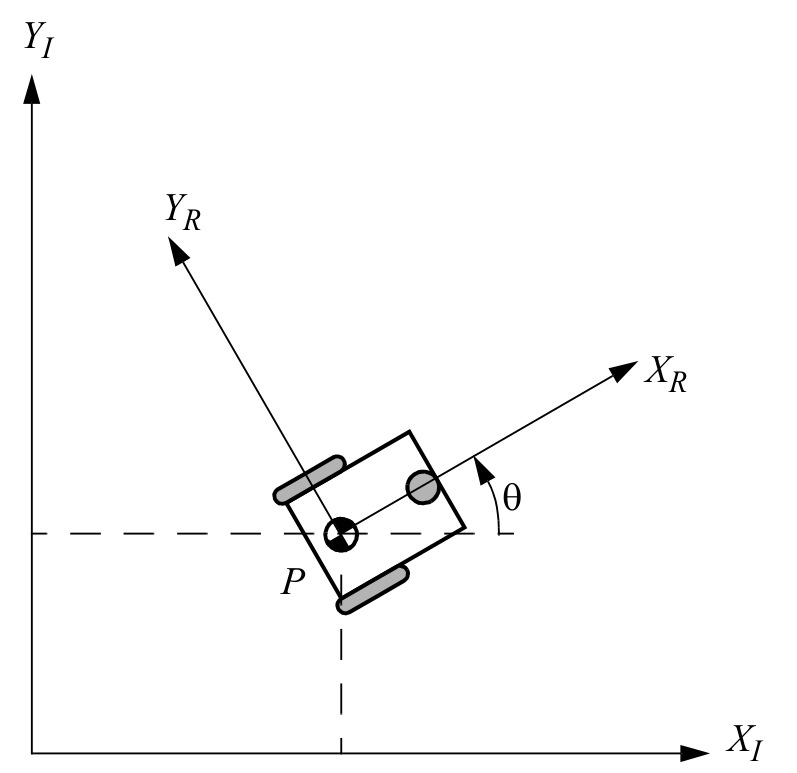
\includegraphics[width=0.4\linewidth]{fk}
    \caption{Forward Kinematics of Mobile Robot \cite{thrun2005probabilistic}.}
    \label{fig:fk}
\end{figure}

Considering the robot from \prettyref{fig:fk}, the position according to the global coordinate system can be represented by $\xi_I = [x, y, \theta]$, as well as the velocity $\dot{\xi} = [\dot{x}, \dot{y}, \dot{\theta}]$. The velocity model for the robot coordinate system can be written as:

\begin{equation}
\dot{\xi_R} = 
\begin{bmatrix}
\cos \theta && \sin \theta && 0 \\
- \sin \theta  && \cos \theta && 0 \\
0 && 0 && 1
\end{bmatrix}
\cdot 
\begin{bmatrix}
\dot{x} \\
\dot{y} \\
\dot{\theta}
\end{bmatrix}
=
R(\theta) \cdot \dot{\xi_I}
\end{equation}

It is easy to calculate the inverse problem using the inverse matrix $R^-1(\theta)$, converting back from the robot coordinate frame to the global frame. The only missing parameter is how the wheel kinematics translate to the $\dot{\xi_R}$ robot velocity, and that will depend on the robot wheel arrangement (wheel type, number of wheels, radius) and the robot dimensions.

The main disadvantages of wheel odometry are that the robot is limited to flat terrain, and even then slippery and small changes to forward kinematics (i.e. radius of the wheel changes slightly) can accumulate error over time, as there is not suitable way to correct the error without other sources of information.

\subsection{Laser Odometry}

Laser odometry bases itself on Laser Scanner data to localize the robot. Instead of using odometry to watch how the robot moves in the environment, it uses the collected data to see how the environment moves in relation to the robot.

One approach to this calculation would be taking two consecutive laser scanners and comparing them. It is assumed that the environment is mostly static so not much should change from one set of data to the other. The transformation that minimizes the distance between points from the two sets is then considered to be movement of the robot in that time slot.

As the small movements are integrated over time, this approach has the same flaws as wheel odometry, with error accumulating over time. However, the robot can improve the accuracy by keeping a laser scanner measurement history and repeating the minimization between many poses. It can also take advantage if it revisits a point in the past where the measurement was more accurate, as it can use data from that measurement for comparison.

\section{The localization and mapping problem}

The localization process can be expressed mathematically as follows \cite{thrun2005probabilistic}. Since all the measurements are discrete and supposing we want the localization of the robot through time, it can be represented as:

\begin{equation}\label{eq:x}
    X_t = \{x_0, x_1, \dots, x_t\} 
\end{equation}

The map can also be represented by a variable M as follows. Notice also that the map is considered to be time invariant in this case, and only depends on $n$ which is the number of features in the world.

\begin{equation}
    M = \{m_0, m_1, \dots, m_{n - 1}\}
\end{equation}

In order to do that, it is necessary to have some idea on how the robot is interacting with the world, how it is moving or the sensors readings. This can be for instance the measurements of robot odometry (wheel or laser odometry) or IMU data. The set of this measurements is defined as:

\begin{equation}
    U_t = \{u_0, u_1, \dots, u_t\}
\end{equation}

To also build the map, the robot will need the set of observations of the world, that can come as measurements from 3D cameras, LIDAR, SONAR, etc. This set of measurements is defined as:

\begin{equation}
    Z_t = \{z_0, z_1, \dots z_t\}
\end{equation}

Since every measurement in the robot is noise, the position can only be represented as a \textit{belief}, where the belief is the probability that the robot is in a position given the set of inputs and measurements. This can be represented as:

\begin{equation}
    bel(x_t, M) = p(x_t, M | u_{1, t}, z_{1,t})
\end{equation}

There are three main approaches to solve this problem, Extended Kalman Filters, Particle Filters and Graph based.

\subsection{Representing the map}

One of the concerns of mobile robots is how to build a map that is compatible with the environment and represents obstacles properly. While in some applications it is possible to have a pre-compiled map from the environment using the floor plan as a reference, those can be obsolete when dealing with highly dynamic environments or when objects get in the way. Even in static environments, there is a need to compensate for faulty or noise sensors, errors in localization, and the pre-compiled maps should only be used as complementary information. One of the techniques that emerged to solve these problems, and later was adopted as the core of many SLAM algorithms, is the Occupancy Grid \cite{elfes1989using} representation.

The Occupancy Grid is form of representing obstacles in 2D or 3D where each cell on the grid stores the probabilistic information of that area. This especially useful because it provides a comprehensive way to fuse sensor data, based on probability, instead of out-of-the-box algorithms that require fine tuning to work.

\begin{figure}[!ht]
    \centering
    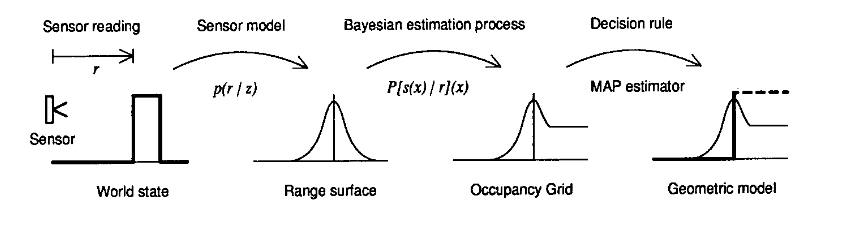
\includegraphics[width=.9\linewidth]{grid_steps}
    \caption{Steps when building an occupancy grid \cite{elfes1989using}.}
    \label{fig:grid_steps}
\end{figure}

According to \prettyref{fig:grid_steps}, the first step when building a sensor grid is to get the sensor reading. The next step is build a sensor model $p(r|z)$. Then, the Bayesian estimation is applied, based on all the observations before and current observations, to update the map. Finally, the world model is obtained using an estimator such as \textit{maximum a posteriori} (MAP). All those steps are done by the SLAM algorithms using different techniques, but even with default tuning those algorithms are good enough to work on most scenarios.

Naturally, the obstacle cell is labeled as occupied, with probability 1. All the cell until this one are labeled as empty, with probability 0. The unknown cells are labeled with unknown, with probability 0.5.

\begin{figure}[!ht]
    \centering
    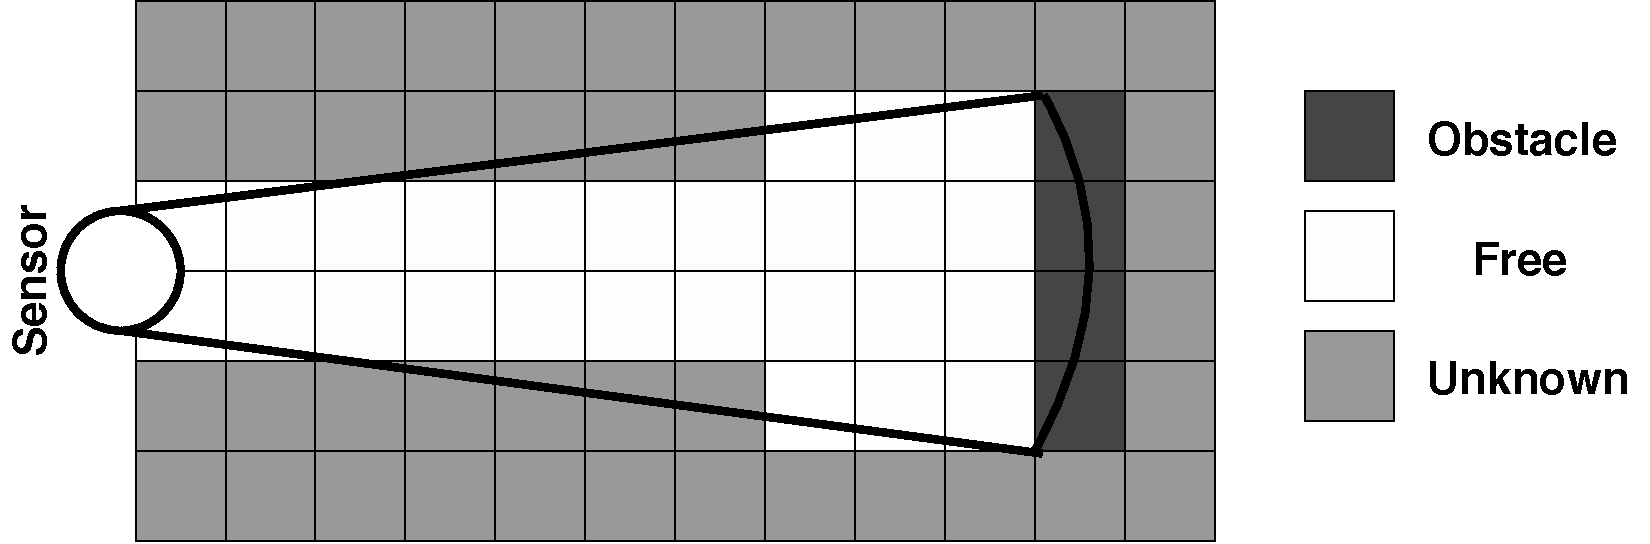
\includegraphics[width=.9\linewidth]{occupancy_grid}
    \caption{Occupancy grid for a single sensor.}
    \label{fig:occupancy_grid}
\end{figure}

The process is iterative and, as measurements from different points of view and different sensors grow, the maps become more and more complete, as shown on \prettyref{fig:occupancy_grid_algorithm}. The data fusion can also be done in different manners, but is commonly done using Kalman filters or Extended Kalman filters.

\begin{figure}[!ht]
    \centering
    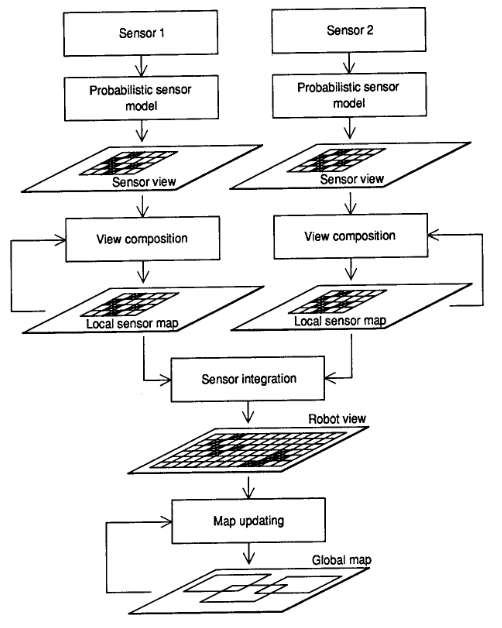
\includegraphics[width=.9\linewidth]{occupancy_grid_algorithm}
    \caption{Occupancy grid algorithm for multiple sensors.}
    \label{fig:occupancy_grid_algorithm}
\end{figure}

\section{ROS Slam Algorithms}

\subsection{Gmapping}

Gmapping is by far the most famous SLAM algorithm in robotics for a number of reasons. It was originally proposed by \citeauthor{doucet2000rao} in 2000 as way of using Particle filters algorithms with Rao-Blackwellized techniques. The main advantage of their approach is dealing with non-gaussian distributions that Kalman filters cannot deal with without rough linearization, as well as being less complex to implement.

\citeauthor{grisetti2007improved} in 2007 proposed improvements to \citeauthor{doucet2000rao} techniques in order to reduce complexity and make the resampling step better. It works by first reducing the amount of particles needed to be stored combining the current observation and odometry information, contrary to previous approaches where only odometry was used, reducing the estimation error and getting a more refined map. The second technique is using an adaptative resampling technique, meaning that resampling only has to be done when needed, reducing the problem with particle depletion, when only few particles are in high-probability areas and a lot of particles represent pretty old and unreliable information.

\subsection{Hector}

Hector SLAM first emerged in 2013 to solve the very specific problem of mapping in uneven terrains. It was aimed to be used in rescue robots that have to be robust enough to drive through ramps and obstacles and still be able to estimate the trajectory and map without reliable odometry information. Instead of trying to filter data to only include useful data, Hector pose estimation completely drops odometry data in favor of laser scanner data, and instead uses a fast LIDAR data scan-matching to estimate odometry. In order to estimate 6DOF, when moving in uneven terrain, the algorithm will also need a IMU device, and optional localization devices  like GPS, barometers and accelerometers. All the data is then fused using an Extended Kalman Filter (EKF), and not including odometry information is a simple way to exclude all errors caused by wheel spin, drift or slippery ground \cite{kohlbrecher2011flexible}.

\subsection{Karto}

Karto is a graph-based SLAM algorithm developed by Karto Robotics and made open-source in 2010. Graph-based SLAM, proposed initially by \citeauthor{lu1997globally}, works by organizing the robot pose information into a graph and then optimizing it to make it more consistent and minimize an error function. While the construction of the graph is heavily sensor dependant, optimizing the graph is computational expensive and the reason why Graph-based SLAM took so long to become popular \cite{grisetti2010tutorial}.

The graph is constructed representing every pose for the robot as a node in the graph. Every robot movement is then represented as an edge in the graph that connect the poses, this data usually being the odometry information. If the robot comes back to a known position, the algorithm does the loop closure and connects the graph to a previously known node. Since the odometry is not reliable, it has to be corrected using the laser scanner measurements. The scan observation in both poses are then matched to calculate the virtual transformation that should map one measurement optimally to the other. Let $z_{i,j}$ be the odometry information between poses $i$ and $j$ and $\hat{z_{i,j}}$ be the expect measurement, the error can be calculated simply subtracting one from the other.

\begin{equation}
    e_{i,j}(x_i, x_j) = z_{i,j} - \hat{z_{i,j}}
\end{equation}

The goal is to ultimately build a function $F(x)$ using the log-likelihood strategy:

\begin{equation}
    F(x) = \sum_{\langle i, j \rangle \ \in \ \mathcal{C}} e_{i,j}^T \Omega_{i,j} e_{i,j}
\end{equation}

so that it can be minimized by the optimization algorithm for $x^*$. In order words, what is the optimal path that minimizes the observed error, given the distribution $\Omega$ and the measurements $z$ and $\hat{z}$.

\begin{equation}
    x^* = \text{argmin}_x \ F(x)
\end{equation}

The optimization is the main problem when dealing with graph-based SLAM, and many different approaches exist to solve this problem. Karto uses Sparse Pose Adjustment, that takes advantage of the sparsity on the large matrices required to solve the problem \cite{konolige2010efficient}.

\subsection{Cartographer}

Cartographer is a fairly recent SLAM technique developed by Google. The concept behind the algorithm can be seen on \prettyref{fig:cartographer}. The main idea is separating the matters into two different problems: local SLAM and Global SLAM. The main objective is not having to deal with big maps or representations while mapping a new area. Instead, a submap is created for the local area and updated every new scan. Every scan is also tested against the submap using a Ceres-based scan matcher, to do pose optimization.

The idea of having submaps is that it is only build using a few scans, meaning that the estimate should be very close to reality. As the submaps grow larger, so does the error, meaning that every few scans a new submap is started. The Global SLAM thread will then have a collection of submaps to compute the whole map running loop closure \cite{cartographer2016google}.

\begin{figure}[!ht]
    \centering
    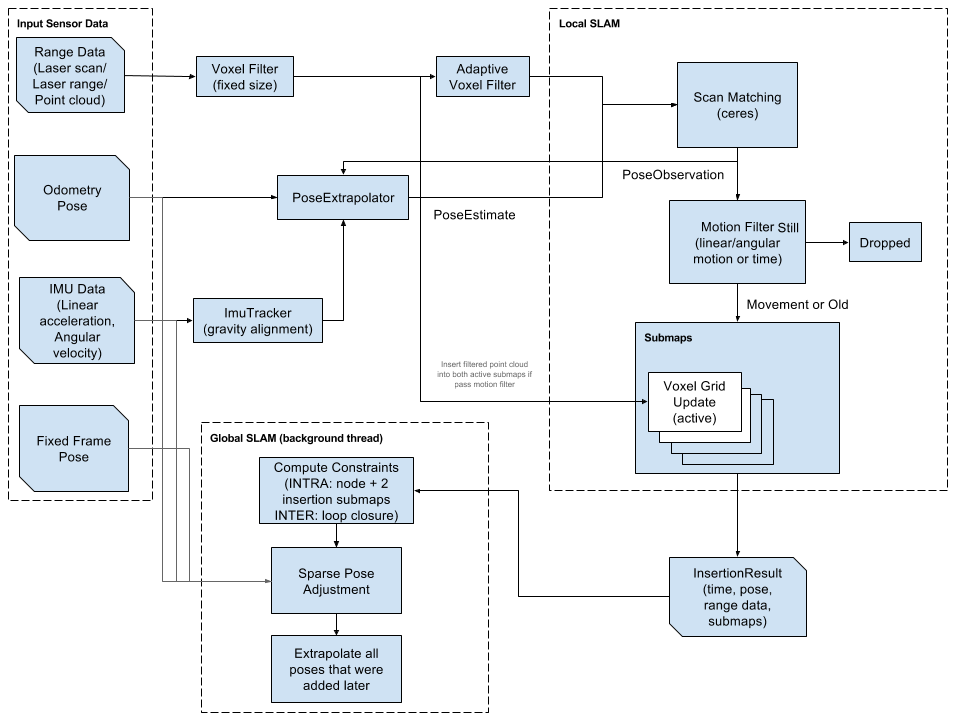
\includegraphics[width=0.6\linewidth]{cartographer}
    \caption{High-level System overview of Cartographer.}
    \label{fig:cartographer}
\end{figure}

\section{Evaluating SLAM Performance}

There is a lot of debate on how to evaluate SLAM performance. Since there are plenty of algorithms using different techniques, each one of the having their own set of parameters, there is a need to inspect them and tell which one does better in each scenario. A lot of this evaluation is done visually, assisted by a human that tells whether the occupancy grid is adequate considering the building floor plans. But as SLAM algorithms gets more precise, it is difficult to draw conclusions just from the appearance itself. Plus, there is the problem of not having the floor plants for publicly available datasets, making it harder to compare between methods \cite{kummerle2009measuring}.

According to \citeauthor{amigoni2007good}, the following issues have to be addressed when comparing SLAM:

\begin{itemize}
    \item The dataset must be pubicly available, examples being MIT Killian Court or the Intel Research Lab dataset.
    \item All algorithm parameters have to be indicated.
    \item The behavior for algorithm have to tested with different parameters in order to evaluate robustness.
    \item The dataset must include a closed-loop test, where the robot runs around an environment and comes back to the same place, to test against algorithm divergence.
    \item The ground truth must be used to evaluate results when available.
    \item Bad mapping results must be shown.
\end{itemize}

The most natural way of analyzing the poses is the squared error from the pose estimates against the ground truth. By calculating the distance from one to another and adding over time, we can get a good metric for the pose error. Considering the $x_i$ as the pose calculated by the SLAM and $x_i^*$ the ground truth pose, we can derive the \prettyref{eq:error_squared} for the squared error.

\begin{equation}\label{eq:error_squared}
\epsilon(x) = \frac{1}{N} \sum_{i}^N (x_i - x_i^*)^2
\end{equation}

\citeauthor{kummerle2009measuring} proposes a framework to analyze mapping accuracy, but uses visual inspection in order to estimate the relations between the robot poses and the environment. The estimation is then compared to the SLAM results and the final metric is the "deformation energy" required to transform the mapped result into ground truth. In other words, each of the $N_c$ displacements $\delta_{i,j}$ is compared against the ground truth $\delta_{i,j}^*$ using the \prettyref{eq:displacement}, for a set of  $(i,j)$ pairs.

\begin{equation}\label{eq:displacement}
    \epsilon(\delta) = \frac{1}{N_c} \sum_{i, j} trans(\delta_{i,j} \ominus \delta_{i,j}^*)^2 + rot(\delta_{i,j} \ominus \delta_{i,j}^*)^2
\end{equation}

 The displacement $\delta_{i, j}$ is simply calculated by the the transformation between a local measurement between two known poses, from pose $x_i$ to pose $x_j$, as described in \prettyref{eq:x}. Evaluating the displacement instead of the global position is great because it makes the evaluation resilient to small errors at the start of mapping that would impact every subsequent global position, even when the mapping in the next steps is done correctly. Since the ground-truth displacement is not available, this implementation relies on the fact that the relation between two poses can be calculated using the laser scanner, each pose later evaluated by a human. It also relies on a good enough initial guess, also human assisted. The authors also assume just evaluating the poses without evaluating the resulting map is enough for SLAM benchmarking. While this hold true for most cases, it is still very hard to infer global performance, as global displacements (large enough distance between $i$ and $j$) also carry the problem of accumulating human error, as each measurement is supervised.
 
 \citeauthor{santos2013evaluation} propose a more in-depth comparison with the publicly available SLAM algorithms that run on ROS. The authors ran both noise-free simulation and real-life experiments with the scenarios and analyzed the error metric between the ground-truth map and the generated map, also evaluating the CPU usage for each algorithm. The authors however didn't provide extensive information on how the maps were aligned, very important since the fit has to be optimal in order to do adequate comparison.
 
 \section{Proposed Evaluation techniques}
 
 In order to better evaluate the algorithms, general guidelines will be respected:
 
 \begin{itemize}
     \item Algorithms available in ROS will be used, to ensure every algorithm is publicly available for testing.
     \item Different maps will be tested to ensure no algorithm is favored. In each run, each algorithm will receive the same working data in the form as ROS bags.
     \item The scenario will be simulated in a map carefully generated using a public tool, to make sure everyone can generate the same testing data. Even though there are differences between simulation and reality, it is the only way to acquire real ground-truth data for the environment.
     \item Maps will test the ability for the algorithm to do accurate mapping, accurate localization and loop-closure. Different measurement techniques will be used to ensure all this three aspects of each map are analysed.
 \end{itemize}
 
The articles discussed already give us a good indication on what to aim for in a comparison algorithm. The first comparison method chosen is the one described in \cite{kummerle2009measuring}, as it best describe local error in the form of displacements when analyzing the trajectory of the robot. Since the ground-truth data is now available and doesn't have to be inferred by a human operator, the process can be done autonomously and we can ensure the data perfectly matches the environment.

The second comparison method chosen is the one demonstrated in \cite{santos2013evaluation}, only that now the approach for lining up the maps and calculating the error metric will be fully described. This approach will help analyzing the quality of the generated map regarding the placement of walls and objects, including their orientation and the amount of noise.

The third metric will focus on analyzing the modeled empty space of each algorithm, to see if the area of the generated room matches the area of the map. This is useful in combination with the last algorithm to see how good is the scale on each map.

\section{Building an accurate map}

It is very important to build accurate maps for SLAM testing, as the resulting map has to be compared against the ground truth and any inaccuracies might lead to different results. For that, a map generation script has been written to generate accurate Gazebo SDF descriptions of the desired map.

To generate a map, we begin with the model we want for the map to be generated with a small image file. As an example, \prettyref{fig:map_generation} is 200x200 pixels. We then draw black pixels that will represent the walls in the generated map. We run the script to generate the map and the result will be something like \prettyref{fig:gazebo_generation}.

\begin{figure}[!ht]
     \centering
     \subfloat[][]{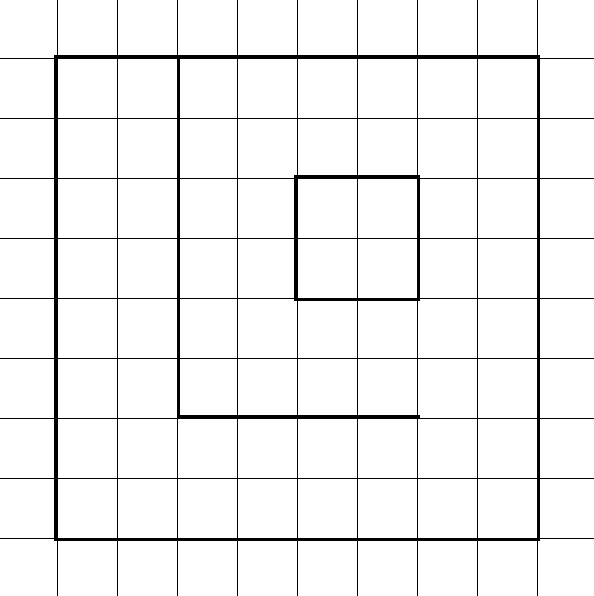
\includegraphics[width=.45\linewidth]{map_generation}\label{fig:map_generation}}
     \hfill
     \subfloat[][]{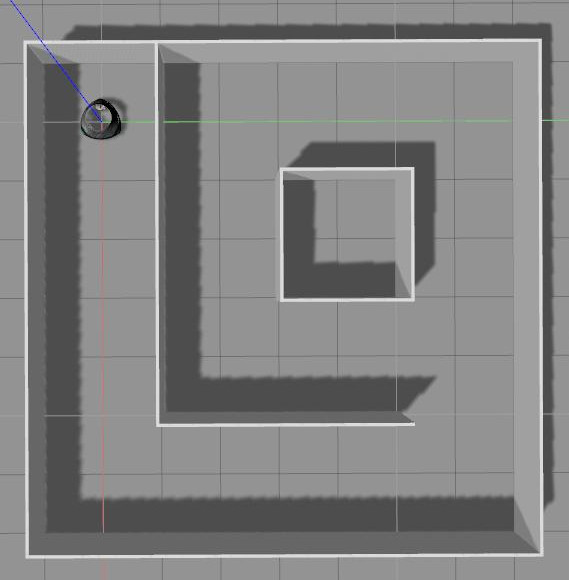
\includegraphics[width=.45\linewidth]{gazebo_generation}\label{fig:gazebo_generation}}
     \caption{Scripted map generation for Gazebo.}
     \label{fig:map_generation_script}
\end{figure}

The main body for the SDF world description can be seen on Listing~\ref{lst:sdf_header}. The only information that has to be filled is the \texttt{\{robot\_start\_pose\}} that will define where the robot will start within the map. The \texttt{\{content\}} tag will then contain a list of walls that compose the test scenario.

\begin{lstlisting}[caption={SDF Header.},label={lst:sdf_header},language=XML]
<?xml version='1.0'?>
<sdf version='1.6'>
    <model name='autogenerated'>
    <pose frame=''>{robot_start_pose} 0 0 0 0</pose>
    
    {content}
    
    <static>1</static>
    </model>
</sdf>
\end{lstlisting} \label{lst:1}

Each wall can be represented by the XML shown in Listing~\ref{lst:sdf_body}. Each will have a unique link name guaranteed by an increasing integer called \texttt{\{link\_number\}}. The \texttt{\{size\}} and \texttt{\{height\}} are the dimensions of the wall. Finally, the \texttt{\{position\}} and \texttt{\{orientation\}} represent the location of the wall center in the world, relative to \texttt{\{robot\_start\_pose\}}.

\begin{lstlisting}[caption={SDF for a single wall.},label={lst:sdf_body},language=XML]
        <link name='Wall_{link_number}'>
            <collision name='Wall_{link_number}_Collision'>
            <geometry>
                <box>
                <size>{size} {height}</size>
                </box>
            </geometry>
            <pose frame=''>0 0 0 0 0 0</pose>
            </collision>
            <visual name='Wall_{link_number}_Visual'>
            <pose frame=''>0 0 0 0 0 0</pose>
            <geometry>
                <box>
                <size>{size} {height}</size>
                </box>
            </geometry>
            <material>
                <script>
                <uri>file://media/materials/scripts/gazebo.material</uri>
                <name>Gazebo/Grey</name>
                </script>
                <ambient>1 1 1 1</ambient>
            </material>
            </visual>
            <pose frame=''>{position} 0 0 0 {orientation}</pose>
        </link>
\end{lstlisting}

\section{Selecting maps}\label{sec:selecting_maps}

The maps have to be selected to be include the scenarios encountered in real life. We selected three maps shown in \prettyref{fig:generated_maps}.

The first map can be seen on \figurename~\ref{subfig:test3}. It is meant to test the loop closure capabilities of each algorithm, since the robot will have to do the full circle and come back to the same point, and then connect the two pathways.

The second map seen on \figurename~\ref{subfig:test2}. It is a more complex version of the first map, and will test the capability of the algorithm to maintain scale between different rooms, as the corridor on the left and the loop on the right are separated by walls.

The third map sown on \figurename~\ref{subfig:test3} will test how the localization performs without revisiting positions, as the robot goes to the center of the loop without previous information and then comes back.

\begin{figure}[!ht]
     \centering
     \subfloat[][]{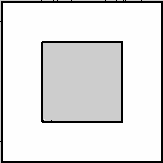
\includegraphics[width=.3\linewidth]{test1}\label{subfig:test1}}
     \subfloat[][]{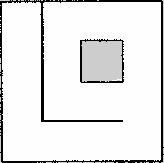
\includegraphics[width=.3\linewidth]{test2}\label{subfig:test2}}
     \subfloat[][]{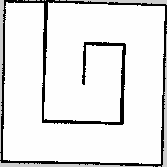
\includegraphics[width=.3\linewidth]{test3}\label{subfig:test3}}
     \caption{Selected maps for testing.}
     \label{fig:generated_maps}
\end{figure}

\section{Setting up the SLAM Algorithms}\label{sec:slam}

The following configuration was used for each of the tested algorithms. If no specified, the default configuration is being used. Cartographer is the only algorithm that also require a Lua file for configuration. All algorithms require the same hardware setup: a source of odometry, in this case a transfomation from the robot fixed frame \texttt{odom\_combined} to \texttt{base\_link} and the laser scanner data, represented by the topic \texttt{scan\_unified} that combines the data from all three lasers scanners on the robot base.

Every output then publishes the calculated map into the \texttt{map} topic and a correction of odometry using a transformation from \texttt{map} to \texttt{odom\_combined}. This transformation is a small displacement between the two frames to account for errors in the odometry for the robot that accumulate over time and can be reduced by taking the pose corrected by SLAM.

\subsection{Gmapping}

To start Gmapping, we call the launch file shown in Listing~\ref{lst:gmapping}. It starts the node \texttt{slam\_gmapping} from package \texttt{gmapping}. The laser scan topic is remapped to match the robot topic name with the \texttt{remap} tag and the odometry frame is provided as \texttt{odom\_combined}. The \texttt{map\_update\_interval} and number of particles are kept in the default configuration. The \texttt{xmin}, \texttt{xmax}, \texttt{ymin} and \texttt{ymax} are the initial size of the resulting map in meters and won't impact the results, as they are automatically increased if the map needs to be bigger. The \texttt{delta} is the map resolution and is kept at the default value of 0.05 pixels/meter.

\begin{lstlisting}[caption={Gmapping launch file.},label={lst:gmapping},language=XML]
<launch>
  <node pkg="gmapping" type="slam_gmapping" name="slam_mapping" output="screen">
    <remap from="scan" to="scan_unified"/>
    <param name="odom_frame" type="string" value="odom_combined"/>
    <param name="map_update_interval" value="5.0"/>
    <param name="particles" value="30"/>
    <param name="xmin" value="-8"/>
    <param name="ymin" value="-8"/>
    <param name="xmax" value="8"/>
    <param name="ymax" value="8"/>
    <param name="delta" value="0.05"/> <!-- map_resolution -->
  </node>
</launch>
\end{lstlisting}

\subsection{Hector}

The Hector mapping node is started using the launch script in Listing~\ref{lst:hector}, starting the node \texttt{hector\_mapping} from package \texttt{hector\_mapping}. We first remap the laser scan to the right topic and use the adequate frame names for the map, base link and odometry link. The \texttt{pub\_map\_odom\_transform} is set to True to publish the transform from \texttt{map} to \texttt{odom\_combined}. The \texttt{laser\_min\_dist} is set to the minimum value registered for the COB laser scanners.

\begin{lstlisting}[caption={Hector launch file.},label={lst:hector},language=XML]
<launch>
  <node pkg="hector_mapping" type="hector_mapping" name="slam_mapping"    output="screen">
    <remap from="scan" to="scan_unified"/>
    <param name="map_frame" value="map" />
    <param name="base_frame" value="base_link" />
    <param name="odom_frame" value="odom_combined" />
    <param name="pub_map_odom_transform" value="true"/>
    <param name="laser_min_dist" value="0.05">
  </node>
</launch>
\end{lstlisting}

\subsection{Karto}

The Karto mapping node is started using the launch script in Listing~\ref{lst:karto}, starting the node \texttt{slam\_karto} from package \texttt{slam\_karto}. We only have to set the the scan and odometry frames. The \texttt{map\_update\_interval} and \texttt{resolution} are set to the same values as Gmapping.

\begin{lstlisting}[caption={Karto launch file.},label={lst:karto},language=XML]
<launch>
  <node pkg="slam_karto" type="slam_karto" name="slam_mapping" output="screen">
    <remap from="scan" to="scan_unified"/>
    <param name="odom_frame" value="odom_combined"/>
    <param name="map_update_interval" value="5"/>
    <param name="resolution" value="0.05"/>
  </node>
</launch>
\end{lstlisting}

\subsection{Cartographer}

The Cartographer node requires a lot of configuration compared to the other SLAM algorithms. Two separate nodes have to be called at start, as seen in Listing~\ref{lst:cartographer}: the \texttt{cartographer\_node} and \texttt{cartographer\_occupancy\_grid\_node}, both from package \texttt{cartographer\_ros}.

The main Cartographer node does all the sub-map generation, and takes as parameters a Lua file with the algorithm configuration, shown in Listing~\ref{lst:cartographer_lua}. The configuration file uses all the default parameters available in Cartographer example files (in file \texttt{backpack\_2d.lua}), with the exception that the IMU was disabled, since COB doesn't have one. The frames were set accordingly and the option \texttt{provide\_odom\_frame} was set to true to get the map to odometry transform during execution. The laser scan was changed from multi echo laser scan to laser scan.

The second node is the occupancy grid node, that reads data from the sub-map list and republishes into the \texttt{/map} topic as a standard Occupancy Grid message from ROS. The resolution is also set to 0.05 pixels/meter.

\begin{lstlisting}[caption={Cartographer launch file.},label={lst:cartographer},language=XML]
<launch>
  <!-- Arguments -->
  <arg name="configuration_basename" default="cartographer.lua"/>

  <!-- cartographer_node -->
  <node pkg="cartographer_ros" type="cartographer_node" name="slam_mapping"
        args="-configuration_directory $(find cob_bringup_sim)/launch
              -configuration_basename $(arg configuration_basename)"
        output="screen">
    <remap from="scan" to="scan_unified" />
  </node>

  <!-- cartographer_occupancy_grid_node -->
  <node pkg="cartographer_ros" type="cartographer_occupancy_grid_node"
        name="cartographer_occupancy_grid_node"
        args="-resolution 0.05" />
</launch>
\end{lstlisting}

\begin{lstlisting}[caption={Cartographer Lua configuration.},label={lst:cartographer_lua},language=Python]
include "map_builder.lua"
include "trajectory_builder.lua"

options = {
  map_builder = MAP_BUILDER,
  trajectory_builder = TRAJECTORY_BUILDER,
  map_frame = "map",
  tracking_frame = "base_link",
  published_frame = "base_link",
  odom_frame = "odom_combined",
  provide_odom_frame = true,
  use_odometry = false,
  num_laser_scans = 1,
  num_multi_echo_laser_scans = 0,
  num_subdivisions_per_laser_scan = 10,
  num_point_clouds = 0,
  lookup_transform_timeout_sec = 0.2,
  submap_publish_period_sec = 0.3,
  pose_publish_period_sec = 5e-3,
  trajectory_publish_period_sec = 30e-3,
  rangefinder_sampling_ratio = 1.,
  odometry_sampling_ratio = 1.,
  imu_sampling_ratio = 1.,
}

MAP_BUILDER.use_trajectory_builder_2d = true
TRAJECTORY_BUILDER_2D.num_accumulated_range_data = 10
TRAJECTORY_BUILDER_2D.use_imu_data = false

return options
\end{lstlisting}

\section{Collecting data} \label{sec:collecting_data}

For data collection, we first start the robot using the command line. We are using \texttt{cob4-9} to avoid having to load unnecessary parts of the robot like the arms or the cameras.

\begin{verbatim}
roslaunch cob_bringup_sim robot.launch robot:=cob4-9 robot_env:=test1
\end{verbatim}

We then launch the controller to be able to drive the robot around using the keyboard.

\begin{verbatim}
roslaunch cob_teleop teleop_keyboard.launch 
\end{verbatim}

Finally, the data is recorded using the rosbag tool. We obviously need the \texttt{/tf}, \texttt{/tf\_static} and \texttt{/scan\_unified} for the SLAM algorithms. The \texttt{/base\_pose\_ground\_truth} is the ground truth data and will be later on used for comparison between algorithms. The \texttt{/base/twist\_controller/command} and  \texttt{/base/odometry\_controller/odometry} are respectively the commands given by the joystick and the calculated odometry after the command has been executed by the robot, and are recorded for in case the bag files need to be re-executed.

\begin{verbatim}
rosbag record /base/odometry_controller/odometry
              /base/twist_controller/command
              /base_pose_ground_truth
              /scan_unified
              /tf
              /tf_static
\end{verbatim}

The data is recorded into a file that can be played at will and will work as the real robot is sending the scans. This ensure every algorithm will get the same working data in the comparisons.

\section{Running the automated reconstruction}

All the steps required for data parsing by the SLAM algorithms were automated to ensure minimal human interaction is required. Once the data has been collected in the previous step, it can be played using the launch file shown in Listing~\ref{lst:parser}.

First we set the parameters and arguments required. The \texttt{use\_sim\_time} ensures the clock will be used from the bag file, not to get inconsistencies with time. The robot is set to \texttt{cob4-9} because this model model will be uploaded for visualization purposes, and it's not required to run the SLAM. We then select the bag file and the algorithm to run together.

The launch file then calls the mapping algorithm, that will launch one of the files described on \prettyref{sec:slam}. Finally, we call the \texttt{rosbag play} node that will play back data already collected to the algorithm, providing clock with the option \texttt{--clock} and with a delay \texttt{-d 5} of 5 seconds to ensure all nodes are initialized before replaying data.

The last include calls for the RVIZ visualization if requested, as shown on \prettyref{fig:rviz_mapping}.

\begin{lstlisting}[caption={Automated data parser.},label={lst:parser},language=XML]
<launch>

  <!-- First set up sim time -->
  <param name="use_sim_time" value="true" />

  <!-- define arguments -->
  <arg name="robot" default="cob4-9"/>
  <arg name="bag" default="test1"/>
  <arg name="slam" default="gmapping"/>

  <!-- Call mapping -->
  <include file="$(find cob_bringup_sim)/launch/cob_$(arg slam).xml" />

  <!-- Play bag data with clock -->
  <node pkg="rosbag" type="play" name="player" output="screen" args="--clock -q -d 5 $(find cob_bringup_sim)/bags/$(arg bag).bag"/>

  <!-- Show visualization if requested -->
  <arg name="rviz" default="false"/>
  <group if="$(arg rviz)">
    <include file="$(find cob_bringup_sim)/launch/visualization.launch" >
        <arg name="robot" value="$(arg robot)" />
    </include>
  </group>
</launch>
\end{lstlisting}

Then, the automated reconstruction can be called:

\begin{verbatim}
roslaunch cob_bringup_sim parse_data.launch
                          rviz:=true bag:=test1 slam:=gmapping
\end{verbatim}

And that will not only launch the bag data \texttt{test1} running Gmapping but also launch a visualization tool to see progress, as shown on \prettyref{fig:rviz_mapping}. The point cloud data resulting from the laser scanners (in red) will be fed to the algorithms and the resulting map (in gray) will be published on the \texttt{map} topic. Every algorithm also publishes the transform from \texttt{map} to \texttt{odom\_combined}.

\begin{figure}[!ht]
    \centering
    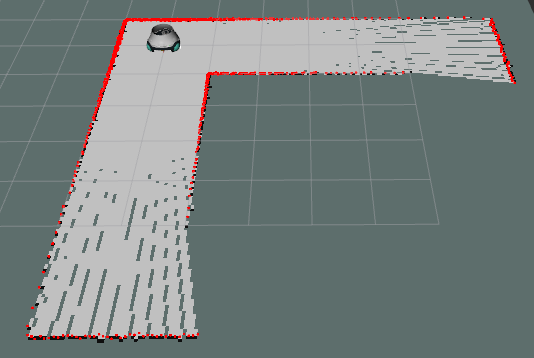
\includegraphics[width=.6\linewidth]{rviz_mapping}
    \caption{Running the automated parser node with Gmapping.}
    \label{fig:rviz_mapping}
\end{figure}

\section{Parsing the data}

The data parser is a Python node that will calculate the required metrics. It runs alongside the SLAM algorithm and constantly import its information. When shut down, the node outputs the desired graphs and metrics. It can be called using the command:

\begin{verbatim}
rosrun cob_bringup_sim pipeline.py
\end{verbatim}

The node keeps executing the following tasks in parallel:

\begin{itemize}
    \item Republishes the ground truth from the ground truth topic (\texttt{/base\_pose\_ground\_truth}, as described in \prettyref{sec:collecting_data}) and republishes it as a tf, since it's easier to do transformations on.
    \item Reads the tf topic and stores a new pose into a pose history whenever the SLAM pose is updated, as well as the ground truth pose.
    \item Collects data from CPU Usage and Memory Usage with the interval of 0.1 seconds.
\end{itemize}

When the node is shutdown, the following tasks are executed:

\begin{itemize}
    \item The pose history is plotted alongside the ground truth.
    \item The squared pose error is calculated according to \prettyref{eq:error_squared}.
    \item The displacement pose error is calculated according to \prettyref{eq:displacement}.
    \item The CPU and Memory usage are plotted over time, using \texttt{psutil} library \cite{psutil}.
    \item The summary is generated including: the average CPU usage, average Memory usage, translation displacement error, rotation displacement error, translation squared error, rotational squared error.
\end{itemize}

\section{Exporting the map}

The map can be exported using the the \texttt{map\_saver} node from the package \texttt{map\_server}. To export the map, simply call the node with the option \texttt{-f} and the map name.

\begin{verbatim}
rosrun map_server map_saver -f map_name
\end{verbatim}

Since Cartographer uses a different approach for generating submaps, the data has to be saved as a \texttt{.pbstream} first to generate the full map. To generate the map, we first have to tell the node to finish the trajectory calling the \texttt{/finish\_trajectory} service. Then, we export the \texttt{.pbstream} file and use it to generate the map. The following sequence of commands represent this process:

\begin{verbatim}
rosservice call /finish_trajectory 0
rosservice call /write_state "filename: '${HOME}/file.pbstream'"
rosrun cartographer_ros cartographer_pbstream_to_ros_map 
       -pbstream_filename ${HOME}/file.pbstream
\end{verbatim}

Because the resulting map doesn't always have the right size (approximately same as the ground truth map), we have to crop the empty gray areas before running the map comparisons. We also want to convert from \texttt{.pgm} saved automatically to \texttt{.png} that the algorithm expects. To do that, we simply call the conversion function from ImageMagick. Why the image is rotated 90 degrees is explained in the next section.

\begin{verbatim}
convert -rotate 90 map_name.pgm -trim map_name.png
\end{verbatim}

\section{Running ICP on resulting map}

Once the map is saved, we have both the reference map and the generated map, as shown in \prettyref{fig:reference_map_icp}. We can then run an algorithm to align the maps properly, as suggested by \citeauthor{santos2013evaluation}.

\begin{figure}[!ht]
     \centering
     \subfloat[][]{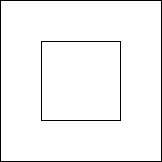
\includegraphics[width=.3\linewidth]{test1_cropped}\label{subfig:test1_cropped}}
     \hspace{2cm}
     \subfloat[][]{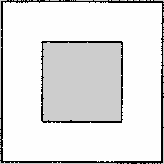
\includegraphics[width=.3\linewidth]{gmapping_test1}\label{subfig:test1_gmapping}}
     \caption{Ground truth (left) and SLAM generated map (right).}
     \label{fig:reference_map_icp}
\end{figure}

First, both maps are imported as a point cloud, each pixel representing a point in space, as shown in \prettyref{fig:point_cloud}. As you can probably tell, the image is twisted 90 degrees counter-clockwise when being read by the algorithm. This happens because the coordinate system for images is not the same as the Cartesian coordinate system.

\begin{figure}[!ht]
     \centering
     \subfloat[][]{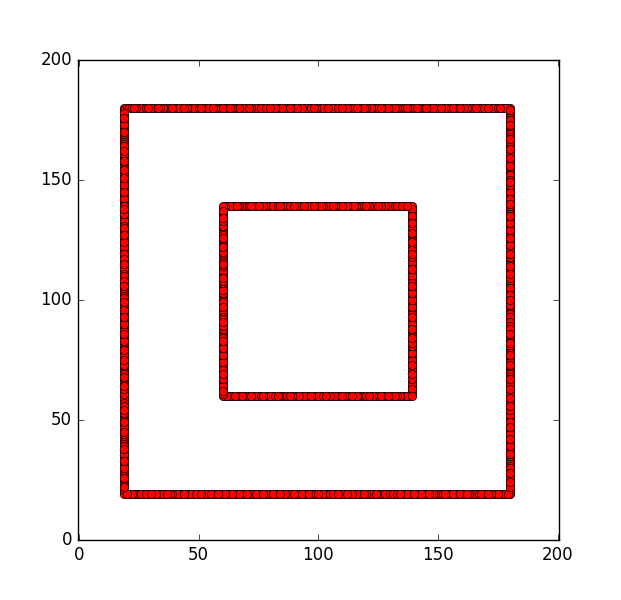
\includegraphics[width=.45\linewidth]{original_pcl}\label{subfig:original_pcl}}
     \hspace{0cm}
     \subfloat[][]{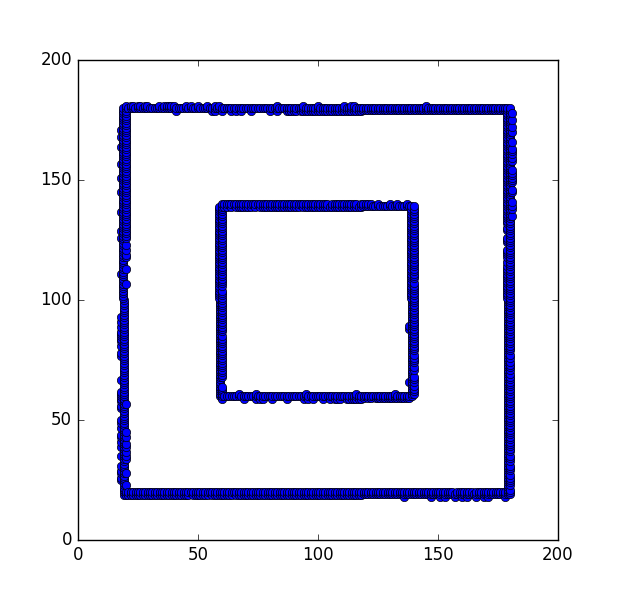
\includegraphics[width=.45\linewidth]{map_pcl}\label{subfig:map_pcl}}
     \caption{Ground truth (left) and SLAM generated map (right) represented in point clouds.}
     \label{fig:point_cloud}
\end{figure}

ICP, or Iteractive Closest Point, is a state-of-the-art way of aligning 3D meshes. It works by finding the transformation that best aligns two distinct point clouds minimizing the error distance between them. For more information about ICP, refer to \citeauthor{besl1992method}.

The ICP algorithm used is the one provided by \citeauthor{flannigan2019}. It will calculate the transformation that best aligns the two maps shown in \prettyref{fig:point_cloud}. With the maps aligned, we then use the following equation to calculate the error metric, where P is the number of points in \figurename~\ref{subfig:map_pcl}, $p_i$ represents one point in the data set and $p_i^*$ is the nearest neighbour of $p_i$ in the dataset shown on \figurename~\ref{subfig:original_pcl}.

\begin{equation}
\epsilon(\text{map}) = \frac{1}{P} \sum_{i=1}^P dist(p_i - p_i^*(p_i))^2
\end{equation}

The aligned point cloud can be seen on \prettyref{fig:alignment_pcl}. To do that, we simply call the node launcher with the desired map and algorithm.

\begin{verbatim}
roslaunch cob_bringup_sim icp_map_comparison.launch map:=test1 slam:=gmapping
\end{verbatim}

\begin{figure}[!ht]
    \centering
    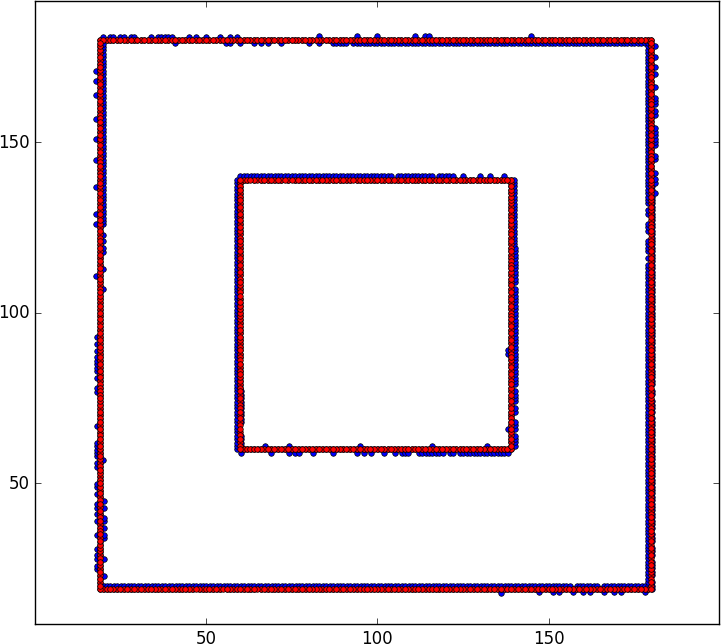
\includegraphics[width=0.45\linewidth]{alignment_pcl}
    \caption{Alignment of point clouds from \prettyref{fig:point_cloud}.}
    \label{fig:alignment_pcl}
\end{figure}

\section{Comparing free space} \label{sec:free_space}

As important as placing the walls in the correct spots, metric that will be checked using ICP, is modeling free space correctly, where the robot can move. This is done by each algorithm by setting the pixels that are free as white. Those white pixels can be counted and checked against the free space in the original map. Since we only want a measurement of scale, we can use the following formula, where $w_o$ is the amount of white pixels in the original image and $w_m$ is the amount of pixels in the map generated by SLAM:

\begin{equation}
\epsilon(\text{space}) = \frac{w_o - w_m}{w_o} \times 100
\end{equation}

The signal of the result will also give indications about the mapping. If it is positive, it means that the original map has more white pixels than the mapped result, meaning the SLAM was more conservative and mapped less space than there is available. If it's negative, the algorithm actually mapped spaced that is not there, meaning the navigation layer will later on have to deal with this problem.